\section{Memory Requirements of Training} \label{sec:2-4-memory-analysis}
In this section, I will show how to perform liveness analysis on an arbitrary computational graph to find the memory allocation strategy that yields the least peak memory.
I will then apply this to the computational graph of training a neural network.
The optimal policy solver for checkpointing presented later will assume these optimisations are in place.

Tim Salimans and Yaroslav Bulatov of OpenAI have a great article online \cite{Bulatov-checkpointing-article} that, with animations, shows how the peak memory of a neural network arises; how to reduce this with checkpointing; and the limitation of chekckpointing to sequences.
I highly recommend reading it.
I borrow from their work in a few sections throughout this thesis, starting here.
I will give a similar analysis of peak memory, but make it more precise for arbtirary costs, and eventually define the exact computation graph that will be used by my policy solver.
In Section \ref{sec:2-5-bg-checkpointing}, I will give a more in-depth discussion of the existing checkpointing techniques, including those already studied in the automatic differentiation literature.
In section \ref{sec:5-qual-eval-seq-only}, I will also show how checkpointing is limited to sequences, as well as reference some recent approaches for tackling this in neural networks.

%%%%%%%%%%%%%%%%%%%%%%%%%%%%%%%%%%%%%%%%%%%%%%%%%%%%%%%%%%%%%%%%%%
\subsection{Pebbling}
Sethi introduced the `pebble game' as a framework for understanding how much memory must be allocated to a computation \cite{Sethi1973}.
In the game, `pebbles' are placed on the nodes, representing their allocation in memory.
The following rules govern the placement of the pebbles:
\begin{enumerate}[topsep=0.1em]
    \item For any \(c = f(a, b)\); \(c\) cannot be computed until both \(a\) and \(b\) have been allocated.
    \item Once no computation relies on \(b\) being in memory, it can be deallocated.
\end{enumerate}
However, these rules allow for many allocation strategies - the order in which we place pebbles, remove them, and reuse them for other nodes.

Consider the following graph in Figure \ref{fig:2-chain-to-pebble}.

\begin{figure}[h]
    \centering
    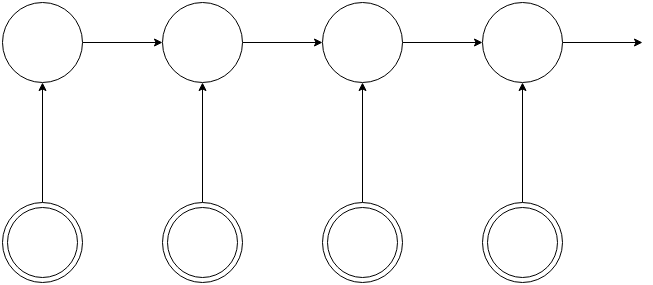
\includegraphics[width=0.5\linewidth]{pebble_chain_1.png}
    \caption{Example graph for pebbling.}
    \label{fig:2-chain-to-pebble}
\end{figure}

One strategy for this graph would be to allocate all the inputs immediately.
This is shown in Figure \ref{fig:2-pebble-chain-bad}.
Coloured nodes are `pebbled' - allocated in memory.

\begin{figure}[hp]
    \centering
    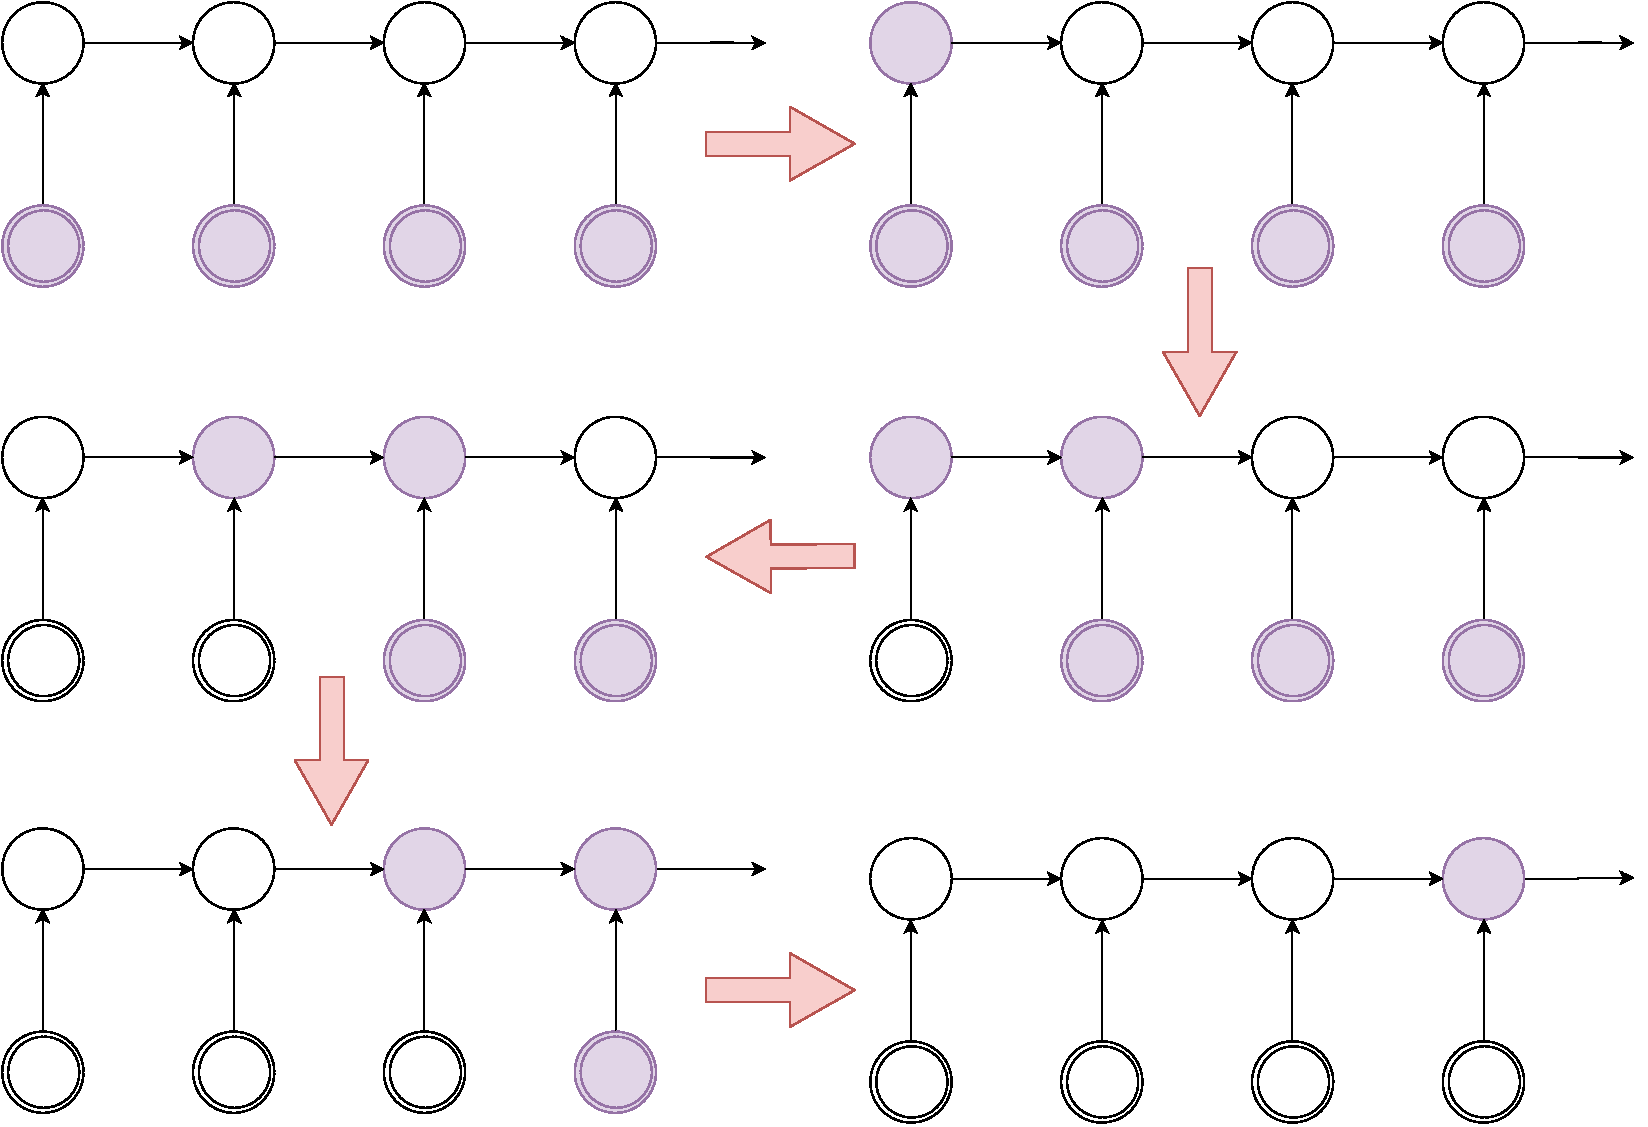
\includegraphics[width=0.95\linewidth]{pebble_chain_2_bad_strat.pdf}
    \caption{A poor pebbling strategy that allocates all leaves immediately. Peak memory is 5 pebbles, occuring in step 2.}
    \label{fig:2-pebble-chain-bad}
\end{figure}

By inspection, we can see the most pebbles (5) are allocated in the second step.
Generalising, for a sequence of size \(n\), \(\Theta(n)\) memory is required.
However, if we instead place pebbles as late as possible, like in Figure \ref{fig:2-pebble-chain-good}, we get a \(\Theta(1)\) strategy.

\begin{figure}[hp]
    \centering
    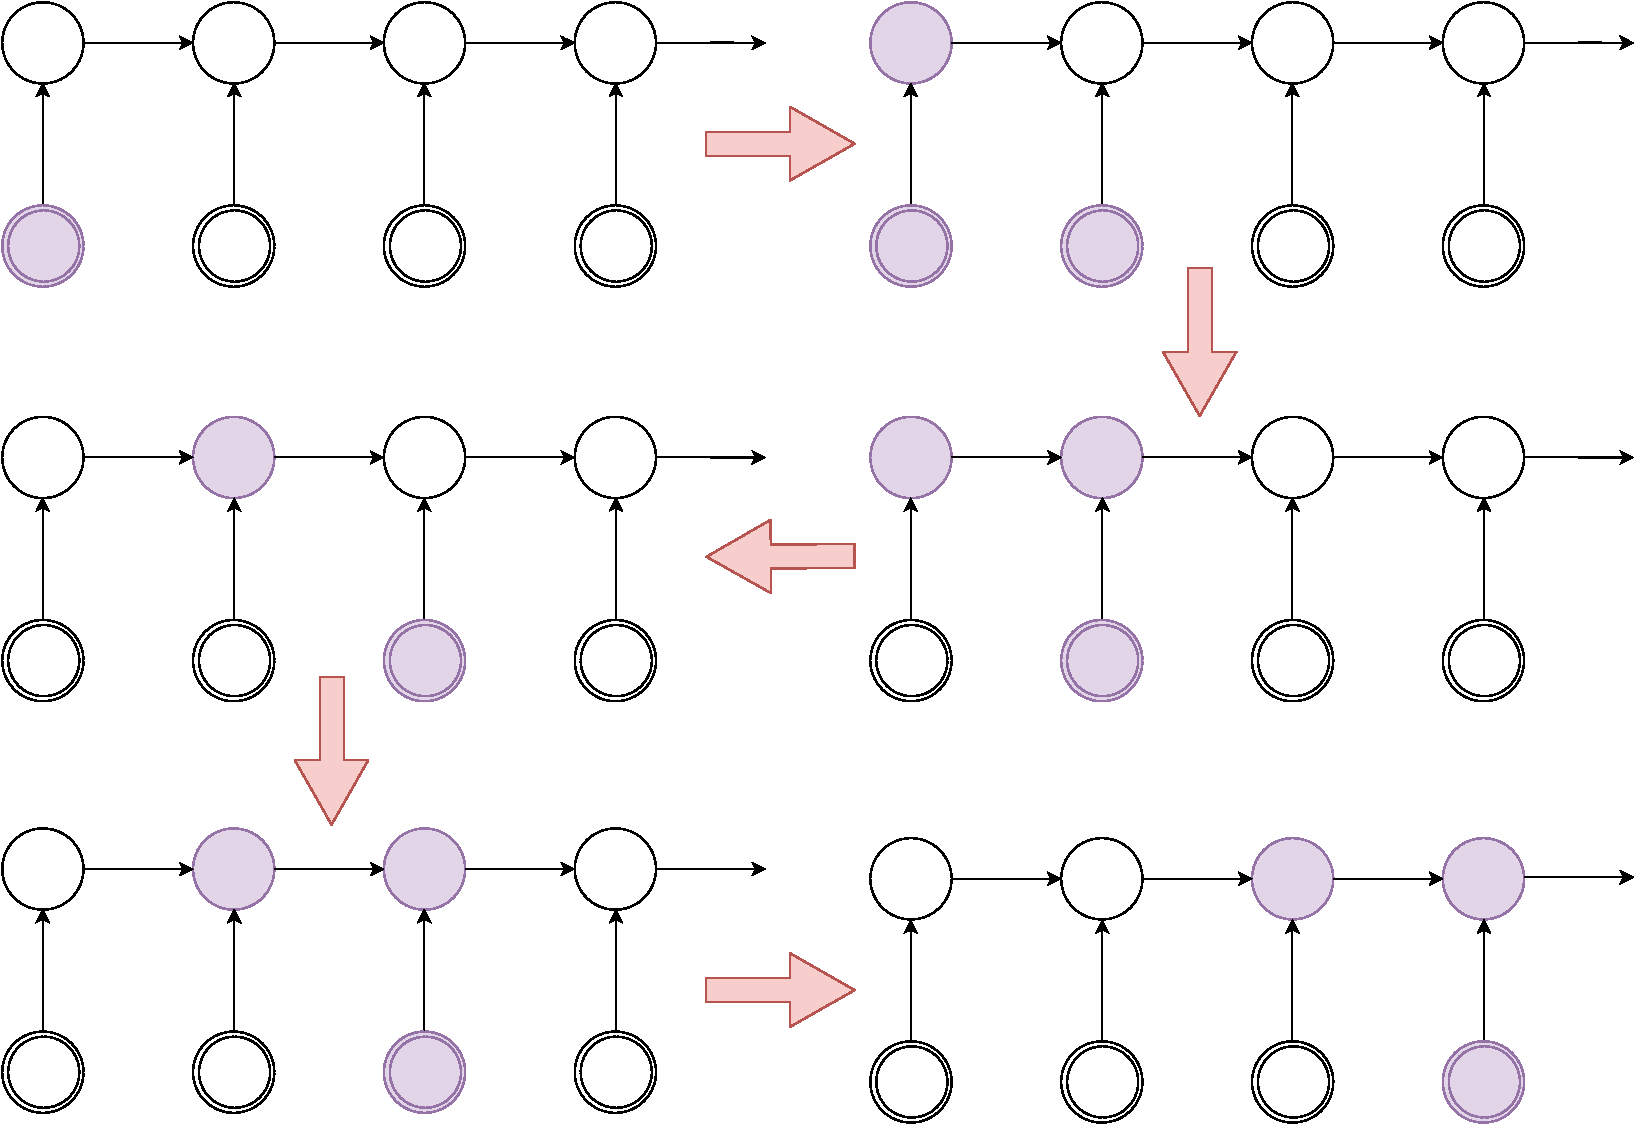
\includegraphics[width=0.95\linewidth]{pebble_chain_3_good_strat.pdf}
    \caption{A good pebbling strategy that allocates leaves lazily. Can handle any chain length with 3 pebbles.}
    \label{fig:2-pebble-chain-good}
\end{figure}

%%%%%%%%%%%%%%%%%%%%%%%%%%%%%%%%%%%%%%%%%%%%%%%%%%%%%%%%%%%%%%%%%%
\subsection{Liveness Analysis}
In general, finding an optimal strategy is hard \cite{Austrin2011}, even in this simplified game where we assume all the nodes have a uniform memory cost.
An example use case is register allocation in compilers \cite{Chaitin1982}.
The first step of register allocation is to determine the lifetimes of each node relative to each other, and thus how their lifetimes overlap.
Variables with overlapping lifetimes cannot be allocated to the same register.
Next, from the liveness analysis, an \textit{interference graph} is constructed.
The nodes of this graph are the variables and they have arcs between them if their lifetimes overlap.
Then, graph colouring is performed.
The colours represent the registers, so this gives an assigment of registers to variables such that no overlapping variables have the same register, using the least amount of registers.

However, this approach takes \(\Theta(n^2)\) to solve, which will be too slow for the size of large neural networks.
We can instead use some reference counting heuristics that are linear time \cite{Chen2016}.
Essentially, we simulate the computation whilst keeping track of, for each node, how many nodes that use it are still yet to be computed. From this, we can perform two optimisations:
\begin{itemize}[topsep=0.1em]
    \item \textbf{Memory Sharing:} Once a node's count has reached zero, it is no longer needed, so its memory can be reused for a different node.
    This simply means we reuse pebbles as soon as they become available.
    \item \textbf{In-place Operation:} When a node's count is one, only one computation depending on it is left.
    That computation can be performed in-place on the already allocated memory.
\end{itemize}
An example of applying these optimisations is shown in Figure \ref{fig:2-chen-LA}.

\begin{figure}[h]
    \centering
    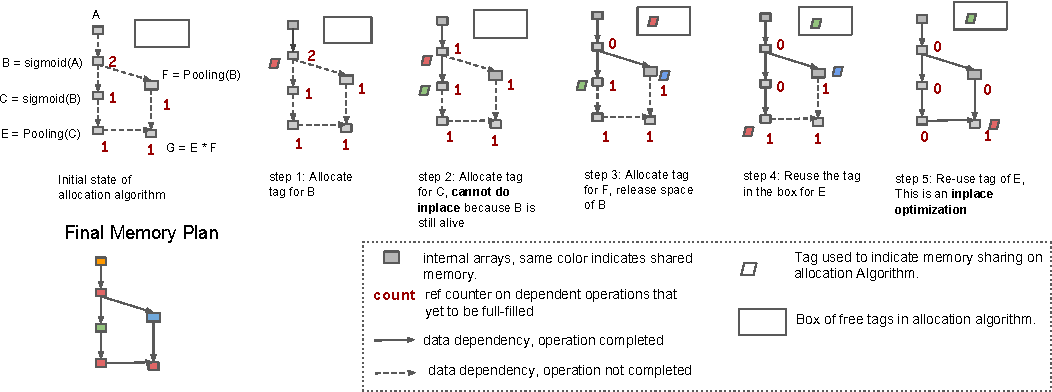
\includegraphics[width=0.97\linewidth]{chen_liveness_analysis.png}
    \caption{Memory allocation algorithm on a computation graph. Each node is associated with a liveness counter to count on operations to be fullfilled. A temporal tag is used to indicate memory sharing. In-place operation can be carried out when the current operations is the only one left (input of counter equals 1). The tag of a node can be recycled when the node’s counter goes to zero. \cite[Figure~2]{Chen2016}}
    \label{fig:2-chen-LA}
\end{figure}

For the examples shown previously, this will find the \(\Theta(1)\) strategy from Figure \ref{fig:2-pebble-chain-good}, in only \(\Theta(n)\) time.

As stated in the whitepaper, PyTorch performs these optimisations aggressively during the backward pass \cite[p.~3]{Paszke2017}.

%%%%%%%%%%%%%%%%%%%%%%%%%%%%%%%%%%%%%%%%%%%%%%%%%%%%%%%%%%%%%%%%%%
\subsection{Peak Memory Usage During Training} \label{sec:2-4-2-peak-mem-training}
Recall the computational graph for one step of training a neural network, repeated in Figure \ref{fig:2-nn-comp-graph-2}.

\begin{figure}[htb]
    \centering
    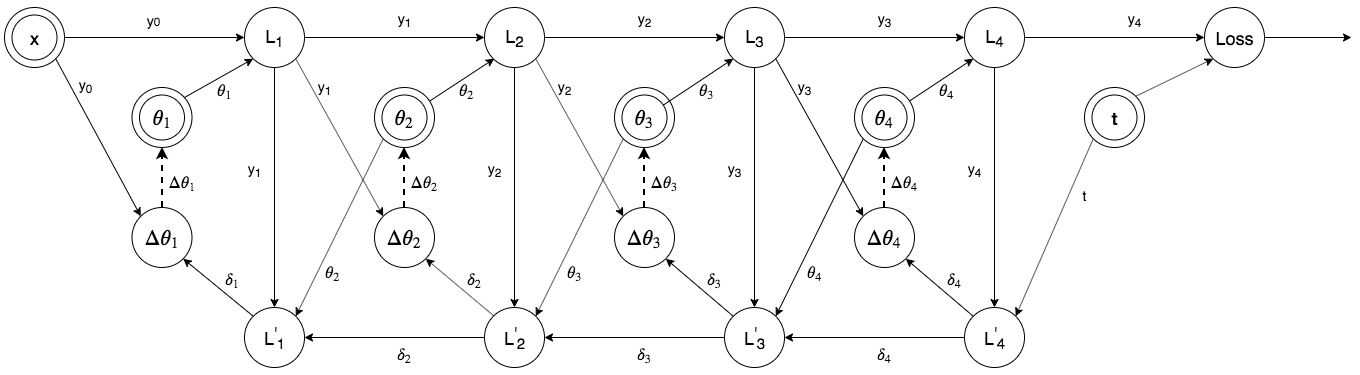
\includegraphics[width=0.97\linewidth]{backprop_full_comp_graph.png}
    \caption{The computational graph for one step of gradient descent on a neural network of four layers.}
    \label{fig:2-nn-comp-graph-2}
\end{figure}

We need to analyse what is actually consuming memory and what is the bottleneck. From the graph, we can see what needs to be allocated:
\begin{itemize}[topsep=0.1em]
    \item The forwards;
    \item The backwards;
    \item The weights;
    \item The targets.
\end{itemize}
However, there is some less obvious memory consumption too.
\begin{itemize}[topsep=0.1em]
    \item \textbf{Workspaces}: Different algorithms for an operator can have different memory requirements. The memory required for an algorithm is known as the workspace.
    \item \textbf{Additional Optimiser Memory}: As mentioned before, in practice vanilla SGD is not used much. Many of the other optimisers require extra memory than just the \(\Delta\theta\). For example they may smooth the update of a parameter by taking some average of the gradient and the previous gradients, in which case the previous gradient must be stored for every parameter.
    \item \textbf{Miscallenous}: The implementation used will likely allocate some miscallenous memory. Between versions of a framework, the exact configuration used, etc., it would be infeasible to account for this statically in a cost model.
\end{itemize}

In my implementation, I will account for the workspace memory as part of the memory required for the forwards and backwards operations.

\begin{figure}[htb]
    \centering
    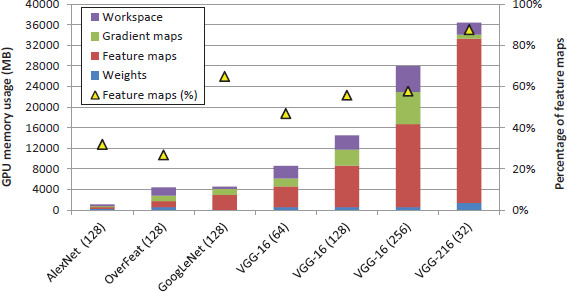
\includegraphics[width=0.7\linewidth]{network_memory_usage_breakdown.jpg}
    \caption{Breakdown of memory usage of popular networks. \cite[Figure~4]{Rhu2016}}
    \label{fig:2-memory-breakdown}
\end{figure}

I will not apply checkpointing to the weights or additional optimiser memory because they only use a small proportion of the total memory reqiurement.
Figure \ref{fig:2-memory-breakdown} shows a break down of memory consumption of popular network architectures.
As can be seen, the proportion of memory allocated to the weights is very small.
The reason is that modern deep networks hardly use fully-connected layers,
which cause an exponential growth in the number of weights.
Instead, we mostly see layers such as the convolutional layer \todo{put in bg}.
These typically apply a small filter, such as of size 3x3, to many large images. \todo{refs?}
The image is the layer output and the filter weights are the learnable parameters.
Thus the parameters are very small compared to the forward and backward tensors.
As the optimiser memory is usually equivalent to one or two extra values \textit{per parameter},
they are omitted from the optimisations too.
%targets? do i omitt them from optimisation, or are they profiled as part of final layer?

Therefore, we can exclude the parameter memory from our analysis.
When checkpointing is applied, it will be assumed that the parameters and their gradients persist in memory throughout the forwards and backwards passes.
However, performing the backwards operators will still involve computing their updates, so the cost of this must be included.
I disucss the modelling of the computational costs because solving for the optimal checkpointing policy requires knowing the per-layer computational costs as well as the memory-costs, since it trades compute for memory.

Omitting the parameters from the computational graph in Figure \ref{fig:2-nn-comp-graph-2} results in the graph typically found in the literature, with some slight tweaks, shown in Figure \ref{fig:2-simplified-comp-graph}.

\begin{figure}[h]
    \centering
    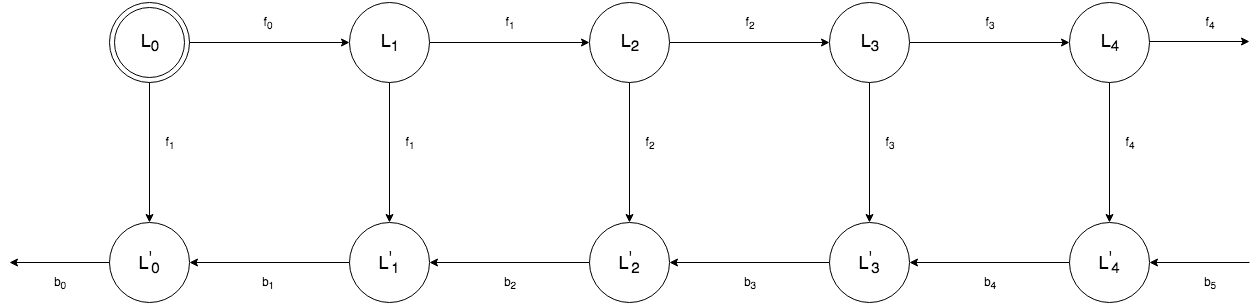
\includegraphics[width=0.9\linewidth]{simplified_comp_graph.png}
    \caption{Computational graph for one step of training, not showing the parameters or their gradients.}
    \label{fig:2-simplified-comp-graph}
\end{figure}

The loss node has also been omitted for brevity.

The forward operators \(L_i\) represent the same forward functions as before.
\(f_{i-1}\) is their input and \(f_{i}\) is their output.
The memory cost of \(f_i\) is modelled as all the (non-parameter) memory required to compute \(y_i\) in the original graph, including the workspace and \(y_i\) itself.
The cost of computing \(f_i\) is just the cost of performing \(L_i\) to get \(y_i\)

The backward operators \(L^\prime_i\) have been defined differently to further simplify the graph. They perform two operations:
(i) using the output of layer \(y_i\) and the upstream backward \(\delta^{i+1}\), compute the upstream weight gradients \(\Delta\theta_{i+1}\); and
(ii) again using the output of layer \(y_i\) and the upstream delta \(\delta^{i+1}\), compute the downstream delta \(\delta^i\).
This means \(L^\prime_{i-1}\) will compute \(\Delta\theta_{i}\).
Consequently, an \(L^\prime_0\) must be added to the graph to represent the computation of \(\Delta\theta_0\).

The memory cost of \(b_i\) is thus all the memory required for \(\delta^i\), but not that for \(\Delta\theta_{i+1}\) as we have excluded parameter memory. However, the computational cost will include the cost to compute \(\Delta\theta_{i+1}\).

\(f_0\) is the inputs. For a network of \(N\) layers, \(f_N\) is the output of the network. \(b_{N+1}\) is the targets. \(b_0\) is not really a tensor that exists; it represents the output of \(L^\prime_{0}\), which is there to set \(\Delta\theta_0\), but does not actually output anything. However, as this incurs some computational cost, which will affect what strategy best optimises the network, we still model this `tensor'.

From here, we can clearly see how peak memory occurs, visualised in Figure \ref{fig:2-nn-peak-mem}.
As the forwards are required again in the backwards pass, they must be kept in memory.
If there were no backwards pass, we could perform all the forwards in-place in \(\Theta(1)\) memory, but instead we must keep them in memory until the backwards pass has used them, resulting in \(\Theta(N)\) memory.
Only once \(b_i\) has been computed, can we finally free \(f_i\) and \(b_{i+1}\).
As a result, peak memory occurs at the end of the forward pass, just before we start backpropagating.

\begin{figure}[hp]
    \centering
    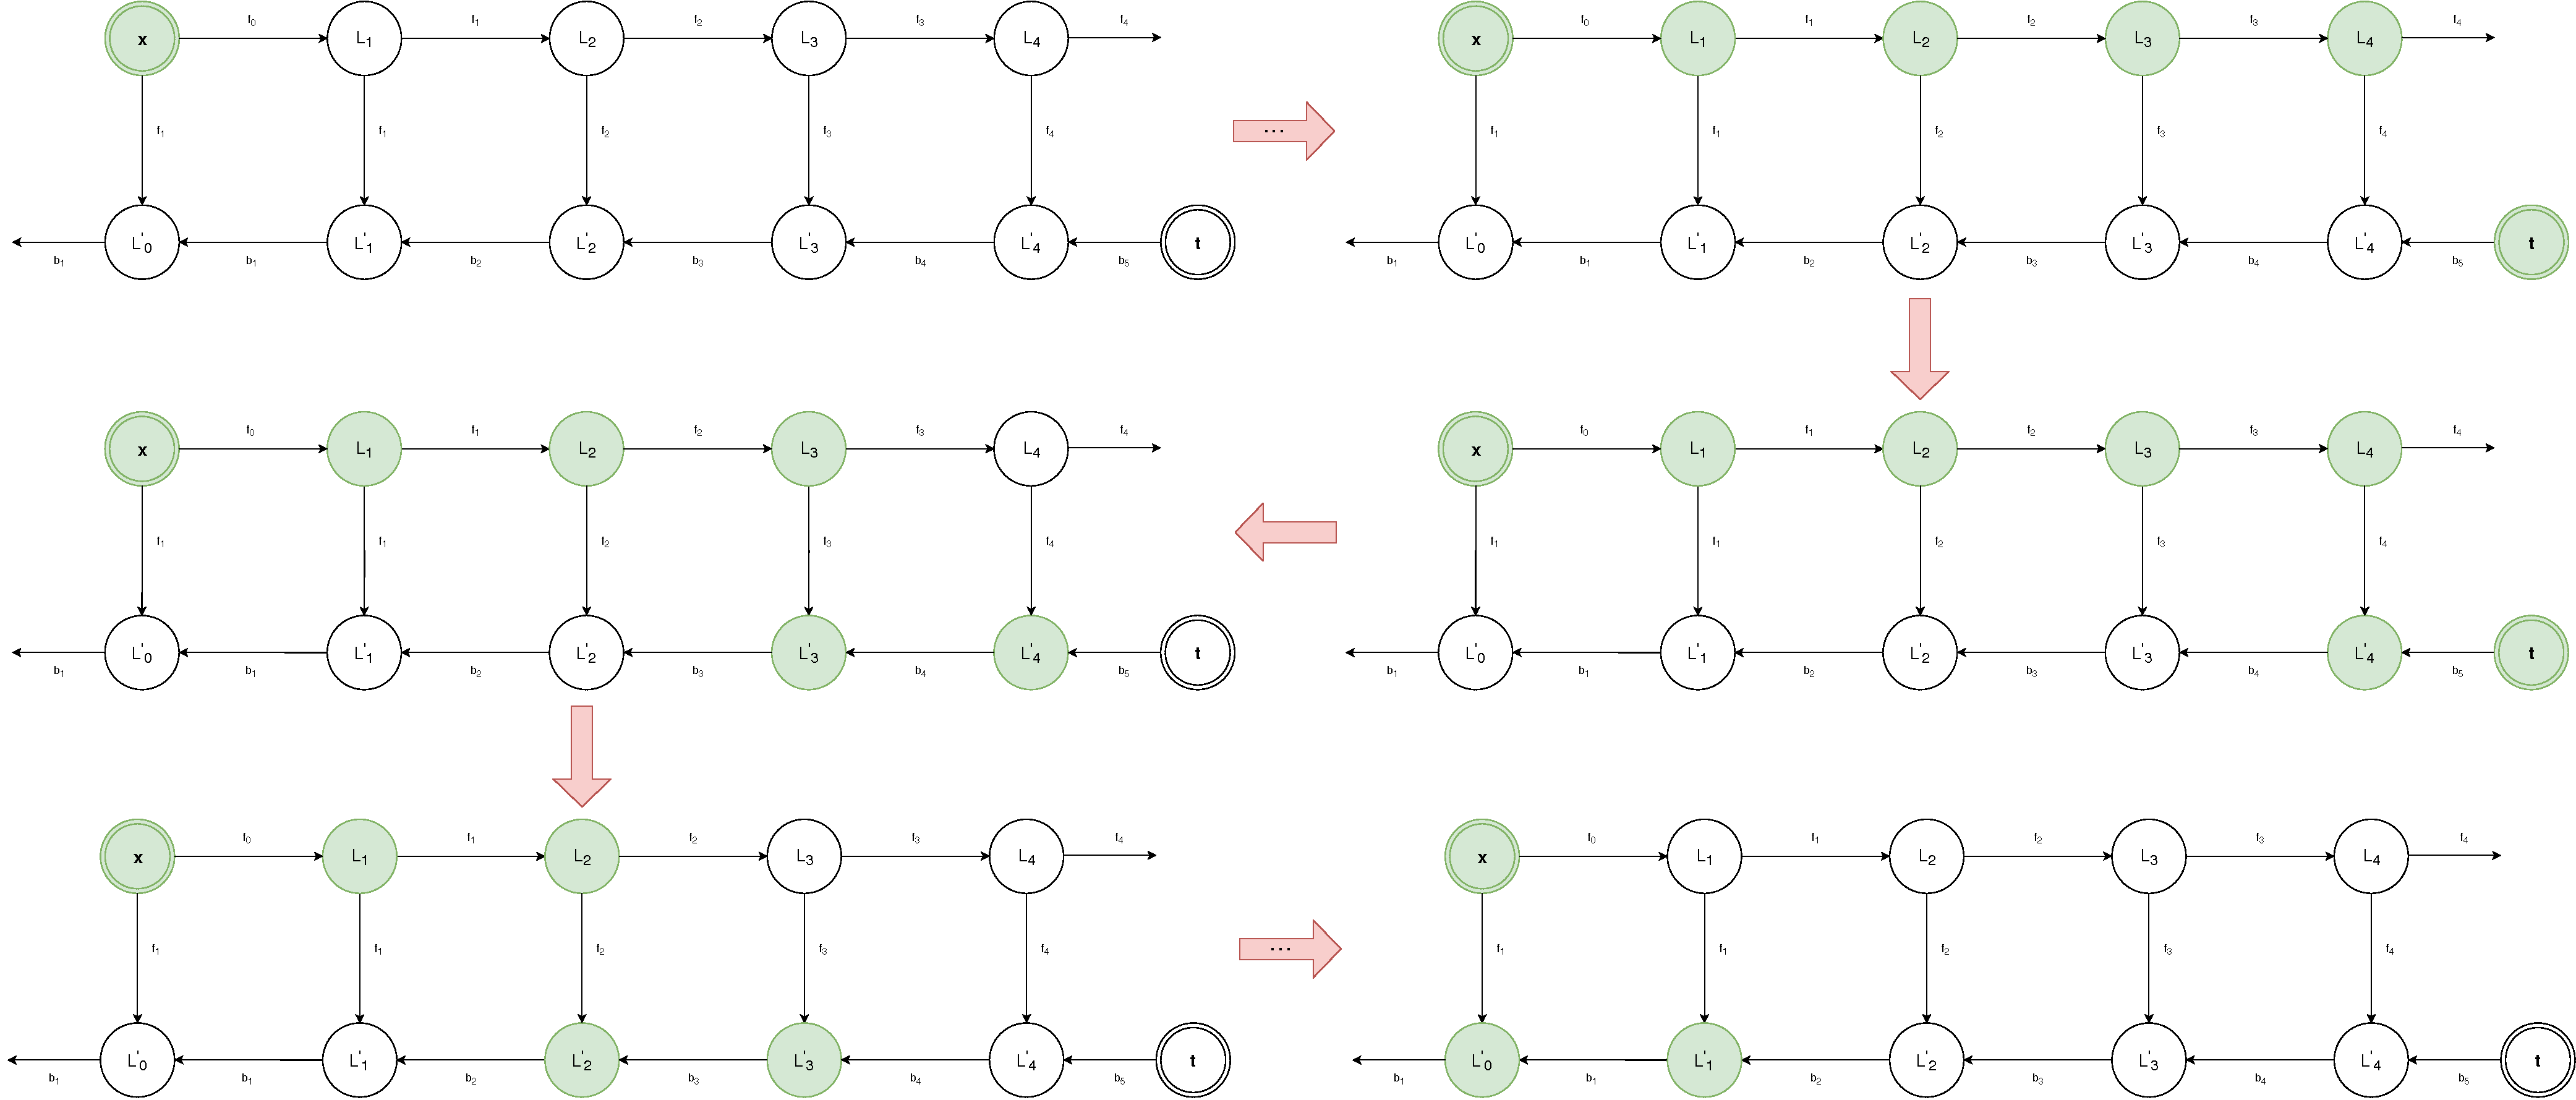
\includegraphics[width=0.95\linewidth]{nn_peak_mem.pdf}
    \caption{Peak memory during backpropagation.}
    \label{fig:2-nn-peak-mem}
\end{figure}

This is the result found in the literature, where per-layer uniform costs are assumed.
However, I am going to be more precise than this;
because the sizes of the tensors vary, peak memory could occur in say the third layer instead of the fourth, if the size of the newly allocated backward is greater than the size of the freed forward and backward together.

Thus, if \(\beta : \{f, b\}\times[0, N] \rightarrow \Z^+\) denotes the memory requirement of the \(i^{\mathrm{th}}\) forward or backward tensor, the peak memory of an N layer network becomes:
\begin{equation}
    \label{eqn:2-nn-peak-mem}
    \max_{0 \leq i \leq N}\; \sum_{l\;=\;0}^i \beta^f_l + \beta^b_{i+1} + \beta^b_i
\end{equation}
